
\chapter{Sound Recording Practice}
\label{examples}

\section{Cable}
\subsection{Unbalanced cable}
An unbalanced audio cdable has two conductors. One carries the audio signal and the other is the shield/ground. 

\subsection{Balanced cable}
Balanced audio requires XLR or TRS connectors with three cables (hot pin 2, cold pin3 and earth 1)
As microphones operate at low voltage levels, it is possible to induce noise in the cable. Balancing a cable gets rid of this noise. A typical balanced cable contains two identical wires, which are twisted together and then wrapped with a third conductor that acts as a shield. One wire is in phase with respect to the source signal, the other wire is reversed in polarity, which is also referred to as being 180 out of phase at all frequencies. The in-phase wire is called non-inverting, positive or ``hot'' while the out-of-phase wire is called inverting, phase-inverted, anti-phase, negative or ``cold''. You have one signal in phase and one out of phase. Since the amplifier at the far end measures the difference in voltage between the two signal lines, noise induced (the same on both signals) is rejected.
 
Therefore your signal voltage is doubled. (Because each wire essentially acts as the reference voltage for the other, with this `equal and opposite' signal format the differential input stage sees a signal which is twice the size of either signal individually: and this gives rise to the often talked about 6dB level hike it produces when compared to connecting the balanced output to an unbalanced destination.)

The theory is based on the Wheatstone Bridge.

\section{Microphones}
Microphones convert sound energy to a changing electric current (a signal).
Main classes of microphones:
\subsection{Dynamic (moving coil) Mics}
\begin{itemize}
\item Low sensitivity because a lot of sound energy is required to move the heavy coil.
\item Usually a very uneven frequency response.
\item Durable - suited to live sound re-enforcement or recording of very loud instruments.
\item Cheap
\end{itemize}

\begin{figure}[H]
\centering
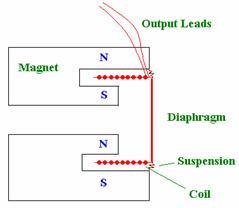
\includegraphics[scale=0.6]{Movingcoil}\caption{Moving coil microphone}
\label{fig:movingcoil}
\end{figure}

\subsection{Condenser (capacitor) Mics}
\begin{itemize}
\item High sensitivity
\item Usually a flatter frequency response
\item Delicate and expensive - damaged very easily so often avoided for live sound re-enforcement.
\item Back Electret - cheaper and usually lower quality then condenser
\end{itemize}


\begin{figure}[H]
\centering
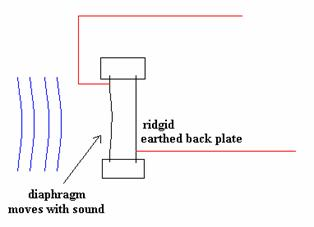
\includegraphics[scale=0.6]{Condenser}\caption{Condenser microphone}
\label{fig:condenser}
\end{figure}

In a typical condenser mic the diaphragm is a very thin circular plate of metal that is free to move. Directly behind the moving plate is a second plate that is fixed. As the moving plate moves due to changes in sound pressure the distance between the plates changes. The two plates form a capacitor (an electronic component that stores charge) and some electronics in the mic turn changing capacitance into changing current (a signal). The electronics needed by the mic require a small amount of power. This is usually provided by phantom power from the preamp (+48v) but can sometimes be a battery in the mic.

\subsection{Ribbon}
\begin{itemize}
\item High sensitivity
\item Usually a flatter frequency response
\item Very expensive and vintage technology.
\item very delicate
\end{itemize}

\begin{figure}[H]
\centering
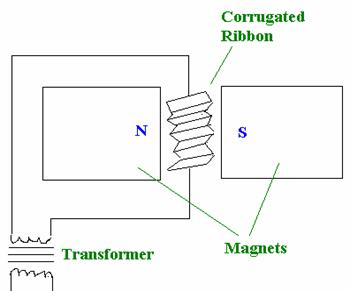
\includegraphics[scale=0.6]{Ribbon}\caption{Ribbon microphone}
\label{fig:ribbon}
\end{figure}

Ribbon mics are very expensive and not that commonly seen but they are usually used when you need a very sensitive pickup. Acoustic instruments etc.

\subsection{Frequency Response}
Microphones and speakers respond differently to specific frequencies.
This response can be shown in a graph of level over frequency.
Sometimes we are interested in a `flat' frequency response. (the unit responds equally to as many frequencies as possible)
Studio loudspeakers almost always aim for the flattest frequency response. Generally this is desirable in a mic as well.
Sometimes we are interested in a characteristic frequency response. (the unit colours the sound by emphasizing or filtering certain frequencies)
Dynamic mics often colour the sound, certain vocal mics aim to produce 'warmer' tones. These mics offer creative possibilities.

\subsection{Polar Patterns}
Microphones have an associated polar pickup pattern. In reality this is frequency dependent (see below) but it is usually generalized into the following:

Omni-directional (equal response in all directions)

\begin{figure}[H]
\centering
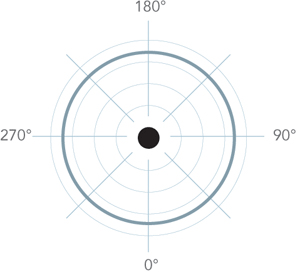
\includegraphics[scale=0.6]{Omni}\caption{Omnidirectional pattern}
\label{fig:omni}
\end{figure}

Cardioid (weighted response from one direction)

\begin{figure}[H]
\centering
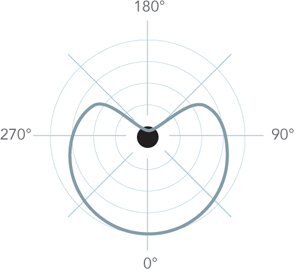
\includegraphics[scale=0.6]{Cardioid}\caption{Cardioid pattern}
\label{fig:cardioid}
\end{figure}

Hyper-Cardioid (more extreme directional variations) (no picture)

Figure eight (bidirectional pickup response, used in M/S pair see below)
\begin{figure}[H]
\centering
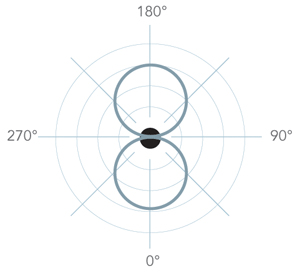
\includegraphics[scale=0.6]{Figureofeight}\caption{Figure 8 pattern}
\label{fig:figure8}
\end{figure}

In reality these pickup patterns extend in 3 dimensions. The following picture highlights this.
\begin{figure}[H]
\centering
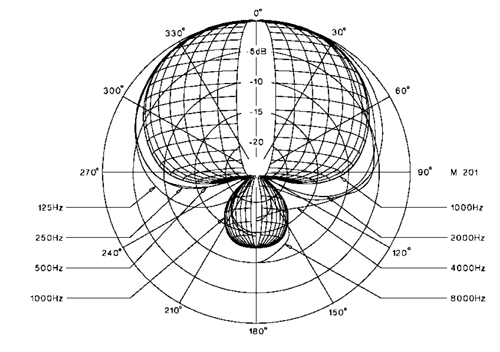
\includegraphics[scale=0.6]{Cardioid3d}\caption{3d cardioid pattern}
\label{fig:3dpattern}
\end{figure}

\subsection{Polar representation of frequency response}

Microphones and loudspeakers have directional characteristics. (They respond differently in different directions)
Most microphone manufacturers provide polar response charts.
Good interactive one at: \href{http://www.neumann.com/?lang=en&id=current_microphones&cid=km180_data#}{Neumann Website}
Learning to read these charts is useful. the following is the frequency response of the D112 kick drum mic.

\begin{figure}[H]
\centering
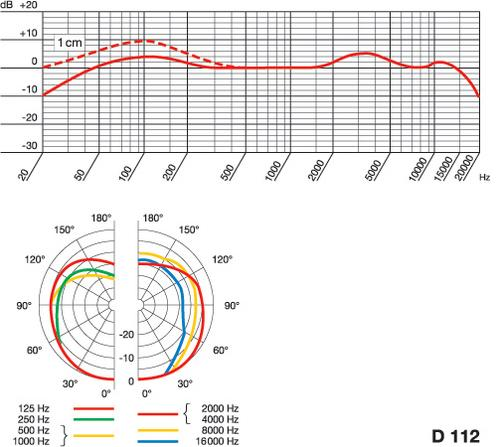
\includegraphics[scale=0.6]{Frequencyresposed112}\caption{Frequency response curve}
\label{fig:freqresponsecurve}
\end{figure}


\section{Capturing a spatial image}
In a recording we will want to recreate the sense of space that was present in the source. We also need to present the recordings through a medium that can reproduce the sense of space. Typically the process is generalised into the term spatial encoding/decoding. We would say that a recording is spatially encoded in stereo, M/S or b-format.

\subsection{Spatial encoding}
Some examples of spatial encoding formats.
\begin{itemize}
\item mono (1 channel)
\item stereo (2 channel, X/Y pair)
\item stereo (2 channel, A/B pair)
\item stereo (2 channel, M/S pair)
\item 4 channel (quad)
\item 4 channel (b-format encoded)
\item 5.1 (5 full range channels and a low frequency effects channel LFE )
\item 7.1 (7 full range channels and a low frequency effects channel LFE )
\item 10.2 (2 * 5.1 rigs at differing altitude)
\item 8 channel (cubic array)
\item 8 channel (circle array)
\end{itemize}

On this course we mainly work in stereo.



\subsection{Stereo capture techniques}

Spaced pair (A/B pair) mics are spaced apart across the sound field

Coincident pair (X/Y pair)

\begin{figure}[H]
\centering
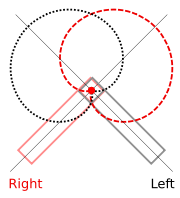
\includegraphics[scale=0.6]{Xypair}\caption{XY pair}
\label{fig:xypair}
\end{figure}

Using figure 8 microphones (therefore capturing more of the room) with conincident spacing (side by side, or one on top of the other) is called a Blumlein pair. 

\begin{figure}[H]
\centering
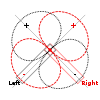
\includegraphics[scale=1.0]{blumleinstereo}\caption{Blumlein pair}
\label{fig:blumleinpair}
\end{figure}

Spaced techniques include:
\begin{itemize}
\item ORTF pair (French Radio), mics spaced 17cm apart at 110 degrees
\item NOS pair (Dutch Radio), mics spaced 30cm apart at 90 degrees
\item RAI pair (Italian Radio), 21cm apart, 100 degrees. 
\end{itemize}

\begin{figure}[H]
\centering
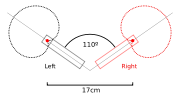
\includegraphics[scale=1.0]{Ortfpair}\caption{ORTF pair}
\label{fig:ortfpair}
\end{figure}

Middle and Side M/S pair
M/S pairs are suited to broadcast because they can be converted to mono without phase cancellations. With this format the spatial information is encoded and must be decoded with the mixer (see diagram) or with a dedicated M/S decoder.

\begin{figure}[H]
\centering
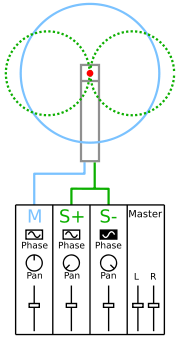
\includegraphics[scale=0.6]{Mspair}\caption{Mid-side pair}
\label{fig:midsidepair}
\end{figure}

Baffled stereo normally uses two omni-directional microphones with an acoustic baffle between them. Microphones are pointed directly at the ensemble and are spaced approximately 35cm apart.

Binaural stereo simulates the human head an usually comprises two omni-directional microphones placed inside a dummy head (and sometimes torso).

Spread stereo techniques can make use of omni or cardioid microphones as required. 

\subsection{Ambisonics}
Ambisonics is a method of capturing the sound in such a way as to preserve as much of the spatial image as possible. The sound is recorded with a special microphone (a sound field mic) and encoded to a 'B-format' stream. The B-format consists of 4 channels: named W, X, Y, and Z. B-format streams can be decoded with some fairly complex mathematics into any arbitrary playback array. So if you have a stereo speaker set it can be decoded to stereo. If you have a home cinema system it can be decoded into 5.1.


Ambisonics encodes sounds from all directions in terms of pressure and velocity components, and decodes these signals to a number of loudspeakers, with psychoacoustically optimised shelf filtering above 700Hz to correct for the shadowing effects of the head. Ambisonics might be considered as the theoretical successor to coincident stereo on two loudspeakers. A good starter reference is Rumsey \citep[pp402-407]{rumsey2006sound} 

USSS has a \href{http://www.core-sound.com/TetraMic/1.php}{TetraMic by Core Sound}
This records A-Format signals (mic pickup) A,B,C and D. The A format consists of the four signals with four sub-cardioid capsules mounted on the four faces of a tetrahedron. So left-front (LF), right-front (RF), left-back (LB) and right-back (RB) (despite them pointing up and down). 

B-format is made up from three figure-eight components (X,Y and Z) and an omni component (W). X is forward facing fig8. Y is sideways fig8. The X, Y and Z components have frontal, sideways and upwards gain of +3dB or root2 with relation to the W signal (0 dB). 

\textbf{Deriving a B format signal from A format}
\begin{verbatim} 
X = 0.5((lf-lb)+(rf-rb))
Y = 0.5((lf-rb)-(rf-lb))
Z = 0.5((lf-lb)+(rb))
W = 0.5(lf+lb+rf+rb)
\end{verbatim} 

To decode into stereo:
\begin{verbatim} 
R = 0.7071 * W + 0.5 * Y
L = 0.7071 * W + -0.5 * Y
\end{verbatim}

To decode into quad:
\begin{verbatim}
R = 0.3536 * W + 0.3536 * X + 0.3536 * Y
L = 0.3536 * W + 0.3536 * X + -0.3536 * Y
RL = 0.3536 * W + -0.3536 * X + 0.3536 * Y
RR = 0.3536 * W + -0.3536 * X + -0.3536 * Y
\end{verbatim}

The full details of this process are here \url{http://www.blueripplesound.com/decoding}


Ambisonics is used mainly in research, particularly the research of spatial sound. The following shows a closeup view of the Soundfield mic capsule and a polar plot of the pickup response of a B-Format stream.


\begin{figure}[H]
\centering
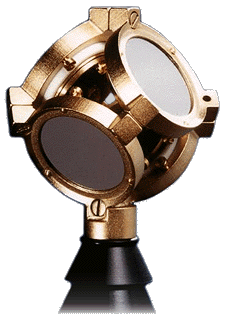
\includegraphics[scale=0.6]{Soundfield}\caption{Soundfield microhpone}
\label{fig:soundfield}
\end{figure}



\begin{comment}

\begin{figure}[H]
\centering
\includegraphics[scale=0.6]{usssinputoutput}\caption{ussstools input output and sfplay}
\label{fig:usssinputoutput}
\end{figure}

\end{comment}
